\documentclass[12pt]{article}

\usepackage[italian]{babel}
\usepackage[T1]{fontenc}
\usepackage{charter}
\usepackage{geometry}
\usepackage{graphicx}
\usepackage{float}
\usepackage{extsizes}
\usepackage{blindtext}
\usepackage{wrapfig}
\usepackage{ragged2e}
\usepackage{xcolor}
\usepackage{subcaption}
\usepackage{keyval}
\usepackage[format=plain, textfont=sl, font=footnotesize]{caption}
\usepackage{hyperref}

\geometry{
 a4paper,
 total={170mm,262mm},
 left=20mm,
 top=20mm,
 }
\graphicspath{ {res/} }
\hypersetup{
    colorlinks = false,
    pdftitle = {Report},
    pdfpagemode=FullScreen,
}
\captionsetup[figure]{labelformat=empty, justification=centering}
\captionsetup[subfigure]{labelformat=empty, justification=centering}
\setlength\intextsep{0pt}
\def\code#1{\texttt{#1}}

\title{Fly Away}
\author{Marco Antolini}

\begin{document}

\topskip0pt
\begin{center}
    \vspace*{\fill}
    \Huge\textbf{Relazione elaborato} \\
    \Huge\textbf{Programmazione di Reti} \\
    \vspace*{\fill}
    \Large{A.A. 2022/2023} \\
    \Large{Traccia 3: Python Web Server} \\
    \vspace*{\fill}
    \Large\textsl{Marco Antolini} \\
    \large\textsl{0000977047} \\
    \large\textsl{marco.antolini6@studio.unibo.it}
    \vspace*{\fill}
\end{center}

\newpage

\tableofcontents

\newpage

% ------------------------------------------------------- ANALISI -------------------------------------------------------

\section{Analisi}

\subsection*{Requisiti}

Si immagini di dover realizzare un Web Server in Python per una agenzia di viaggi.
I requisiti del Web Server sono i seguenti: \\
• Il web server deve consentire l’accesso a più utenti in contemporanea. \\
• La pagina iniziale deve consentire di visualizzare la lista dei servizi
erogati dall’agenzia di viaggi e per ogni servizio avere un link di
riferimento ad una pagina dedicata presente nella stessa working
directory della pagina principale. \\
• Nella pagina principale dovrà anche essere presente un link per il
download di un file pdf da parte del browser. \\
• Come requisito facoltativo si chiede di autenticare gli utenti nella fase
iniziale della connessione. \\
• L’interruzione da tastiera (o da console) dell’esecuzione del web server
deve essere opportunamente gestita in modo da liberare la risorsa
socket. \\
\begin{figure}[h]
    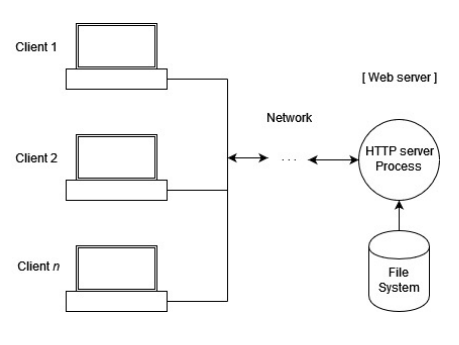
\includegraphics[width=0.5\linewidth]{requisiti.png}
    \centering
\end{figure}
\vskip 1.5cm

% ------------------------------------------------------- PROGETTAZIONE -------------------------------------------------------

\section{Progettazione}

Per la realizzazione del progetto è stato utilizzato il linguaggio di programmazione Python, in particolare grazie all'aiuto della libreria Flask che fornisce un'interfaccia per la creazione di applicazioni web in Python e comprende numerose funzionalità che facilitano la creazione e la gestione di un web server. \\
La libreria Flask comprende al suo interno la libreria Jinja2 che permette di creare template HTML che possono essere utilizzati per la creazione di pagine web dinamiche. \\
Quindi tramite Python ho gestito lo sviluppo del back-end, mentre per il front-end ho utilizzato i template HTML, assieme assieme a CSS puro per la gestione del layout e della grafica e JavaScript per la gestione delle funzionalità dinamiche.

\newpage

% ------------------------------------------------------- Front-End -------------------------------------------------------

\subsection{Front-end}

\subsubsection{Template HTML}

\justifying
Per quanto riguarda il front-end, come introdotto in precedenza, ho usato la libreria Jinja2 (parte di Flask) che permette di creare dei template HTML, che verranno poi caricati dalle funzioni \raggedright di view del back-end.
\begin{wrapfigure}[14]{r}{0.47\linewidth}
    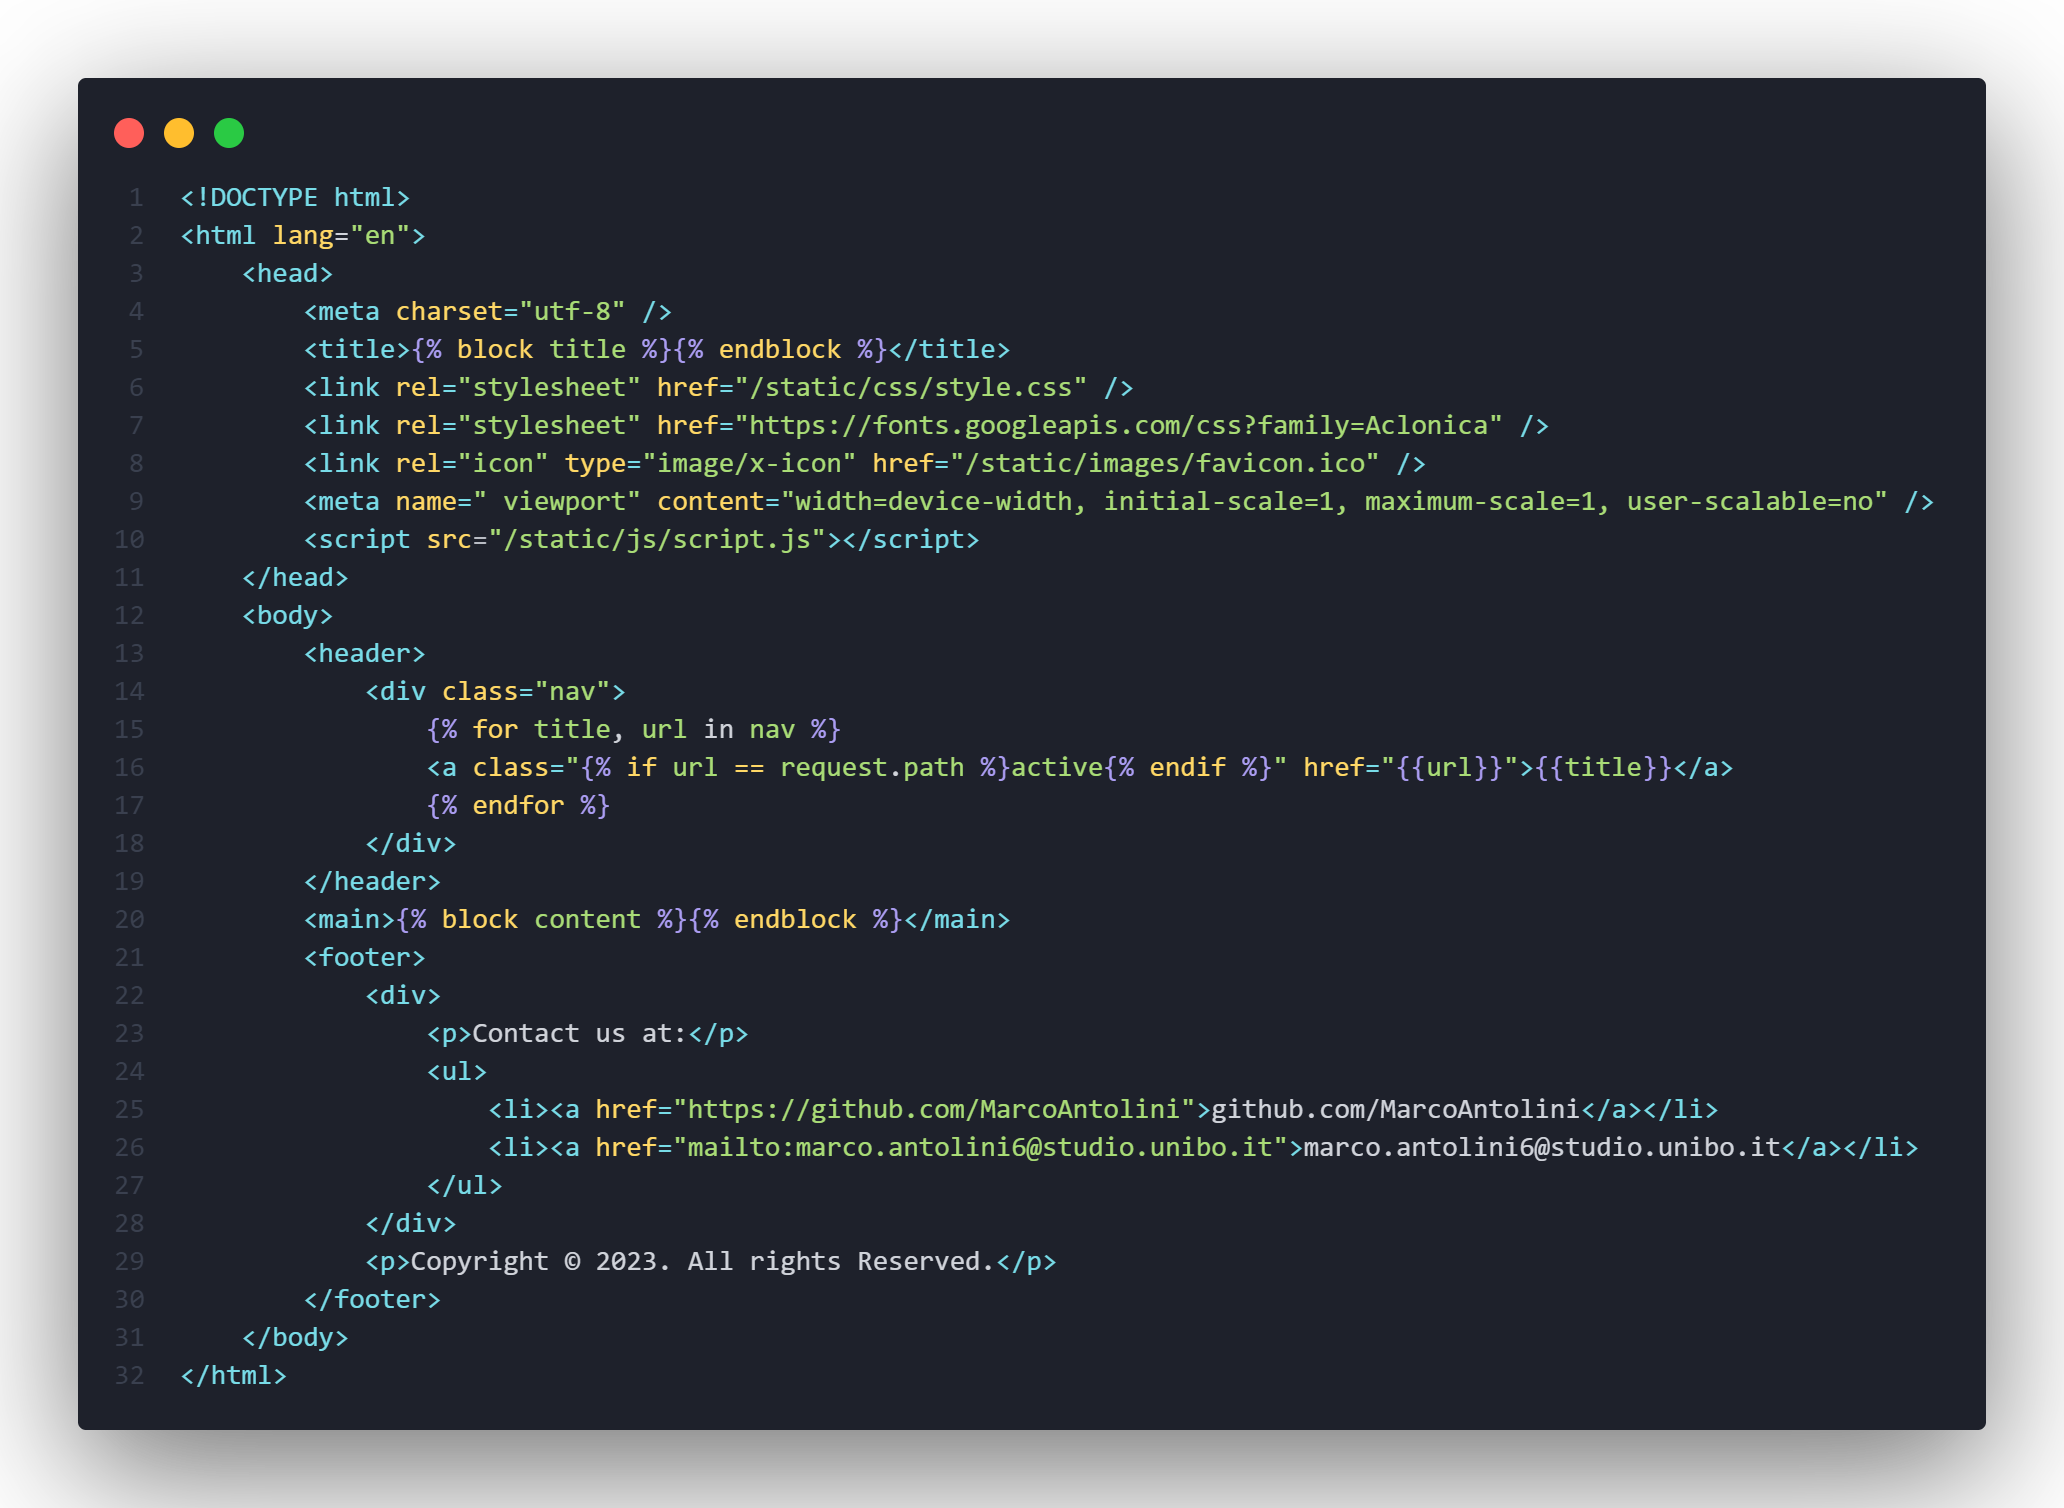
\includegraphics[width=8cm]{base-template.png}
    \caption{Template \code{base.html}}
    \centering
\end{wrapfigure}
\justifying
Jinja2 permette di creare template di base che possono essere estesi e personalizzati per ogni pagina web. Ho quindi creato un template \code{base.html} che contiene la struttura base di ogni pagina web (come ad esempio il layout, il menu di navigazione, il footer, ecc.) e poi ho creato dei template che estendono il template base e che vengono utilizzati per le varie pagine web. \\
Come si può notare nell'immagine è possibile utilizzare del codice python all'interno del template HTML racchiuso all'interno di parentesi graffe \code{\{\}}, questo codice viene poi eseguito dal back-end e il risultato viene poi inserito nel template HTML. Inoltre è possibile notare che possono essere usate delle variabili (come ad esempio \code{request.path}) all'interno del template se opportunamente passate dal back-end. \@

\noindent
\justifying
Il template base al suo interno contiene dei tag \code{block} che vengono poi implementati dai template che estendono il template base e vi accedono grazie al nome assegnato al tag

\noindent\code{block}
\raggedright (nel mio esempio \code{title} e \code{content}).
\begin{wrapfigure}{r}{0.47\linewidth}
    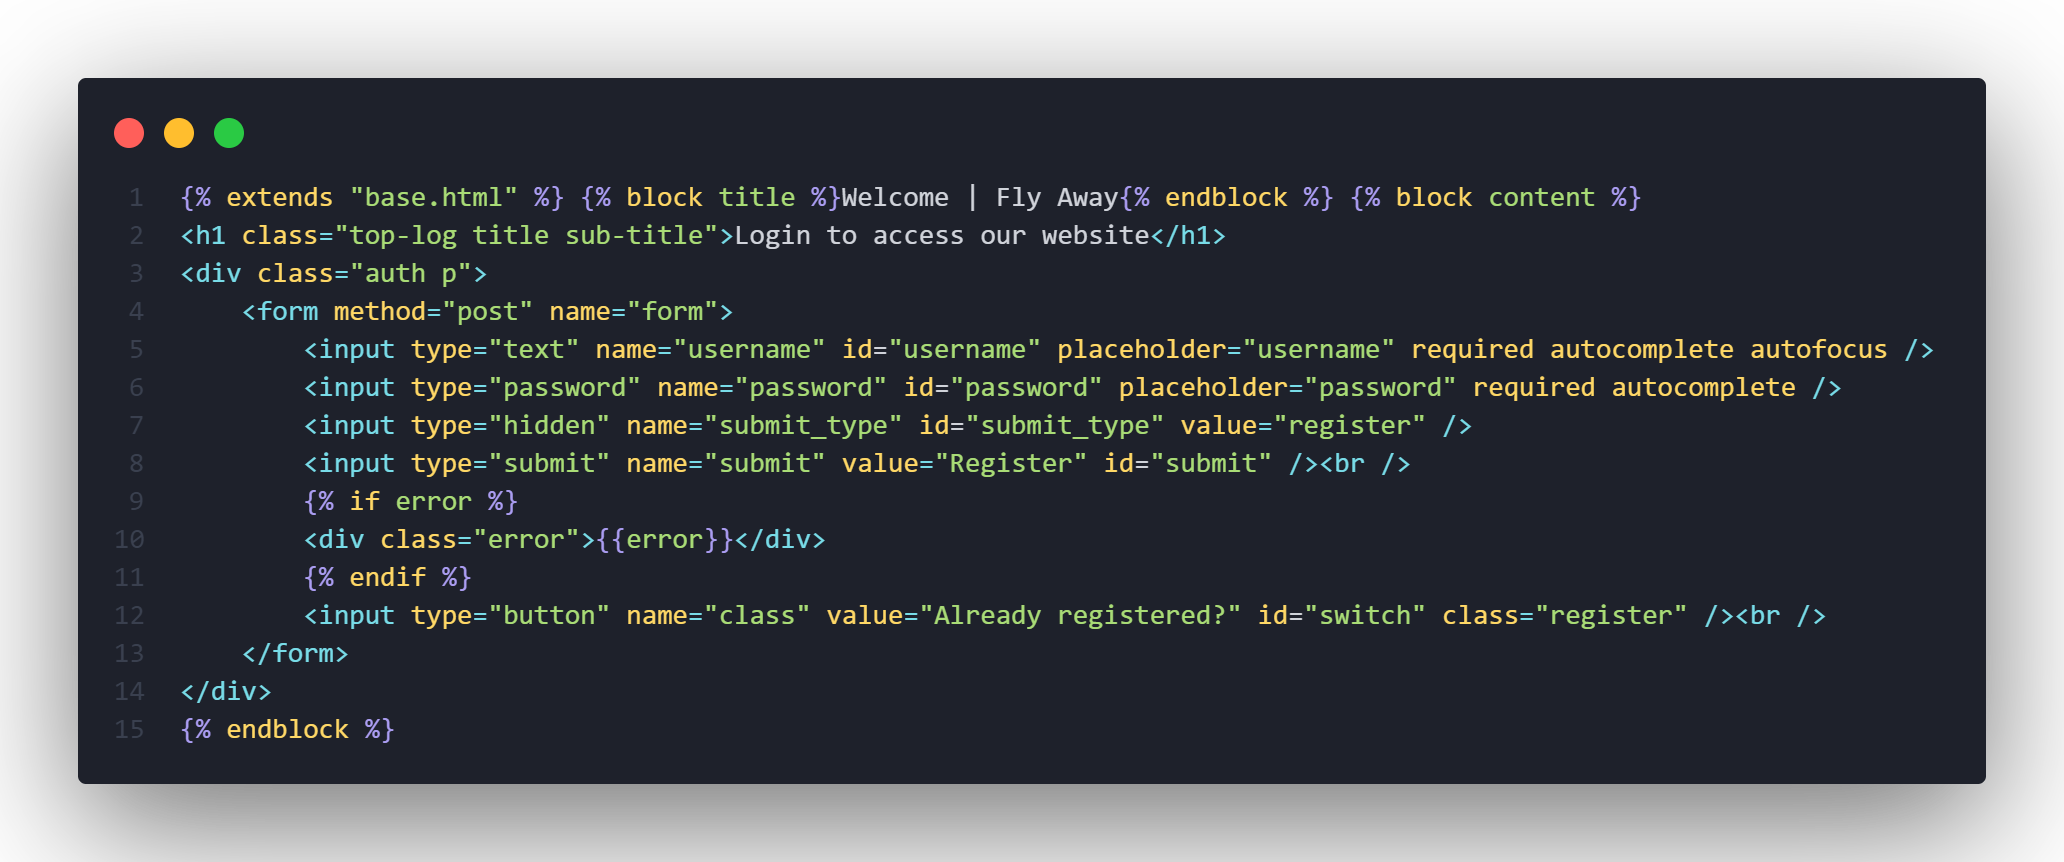
\includegraphics[width=8cm]{extend-template.png}
    \caption{Esempio di template esteso (\code{welcome.html})}
    \centering
\end{wrapfigure}
\justifying
Come si può notare nell'immagine, il template \code{welcome.html} estende il template \code{base.html} e quindi può accedere ai tag \code{block} del template base. Inoltre è possibile notare che è possibile passare delle variabili al template base tramite il tag \code{extends} (nel mio esempio \code{title} e \code{content}). \\

\subsubsection{CSS}

Per quanto riguarda il CSS ho utilizzato solo CSS puro ed esterno (quindi un file \code{style.css} che accede ad ogni elemento grazie al suo tag HTML o alla sua classe), senza utilizzare nessuna libreria o framework. \\
\begin{figure}[h]
    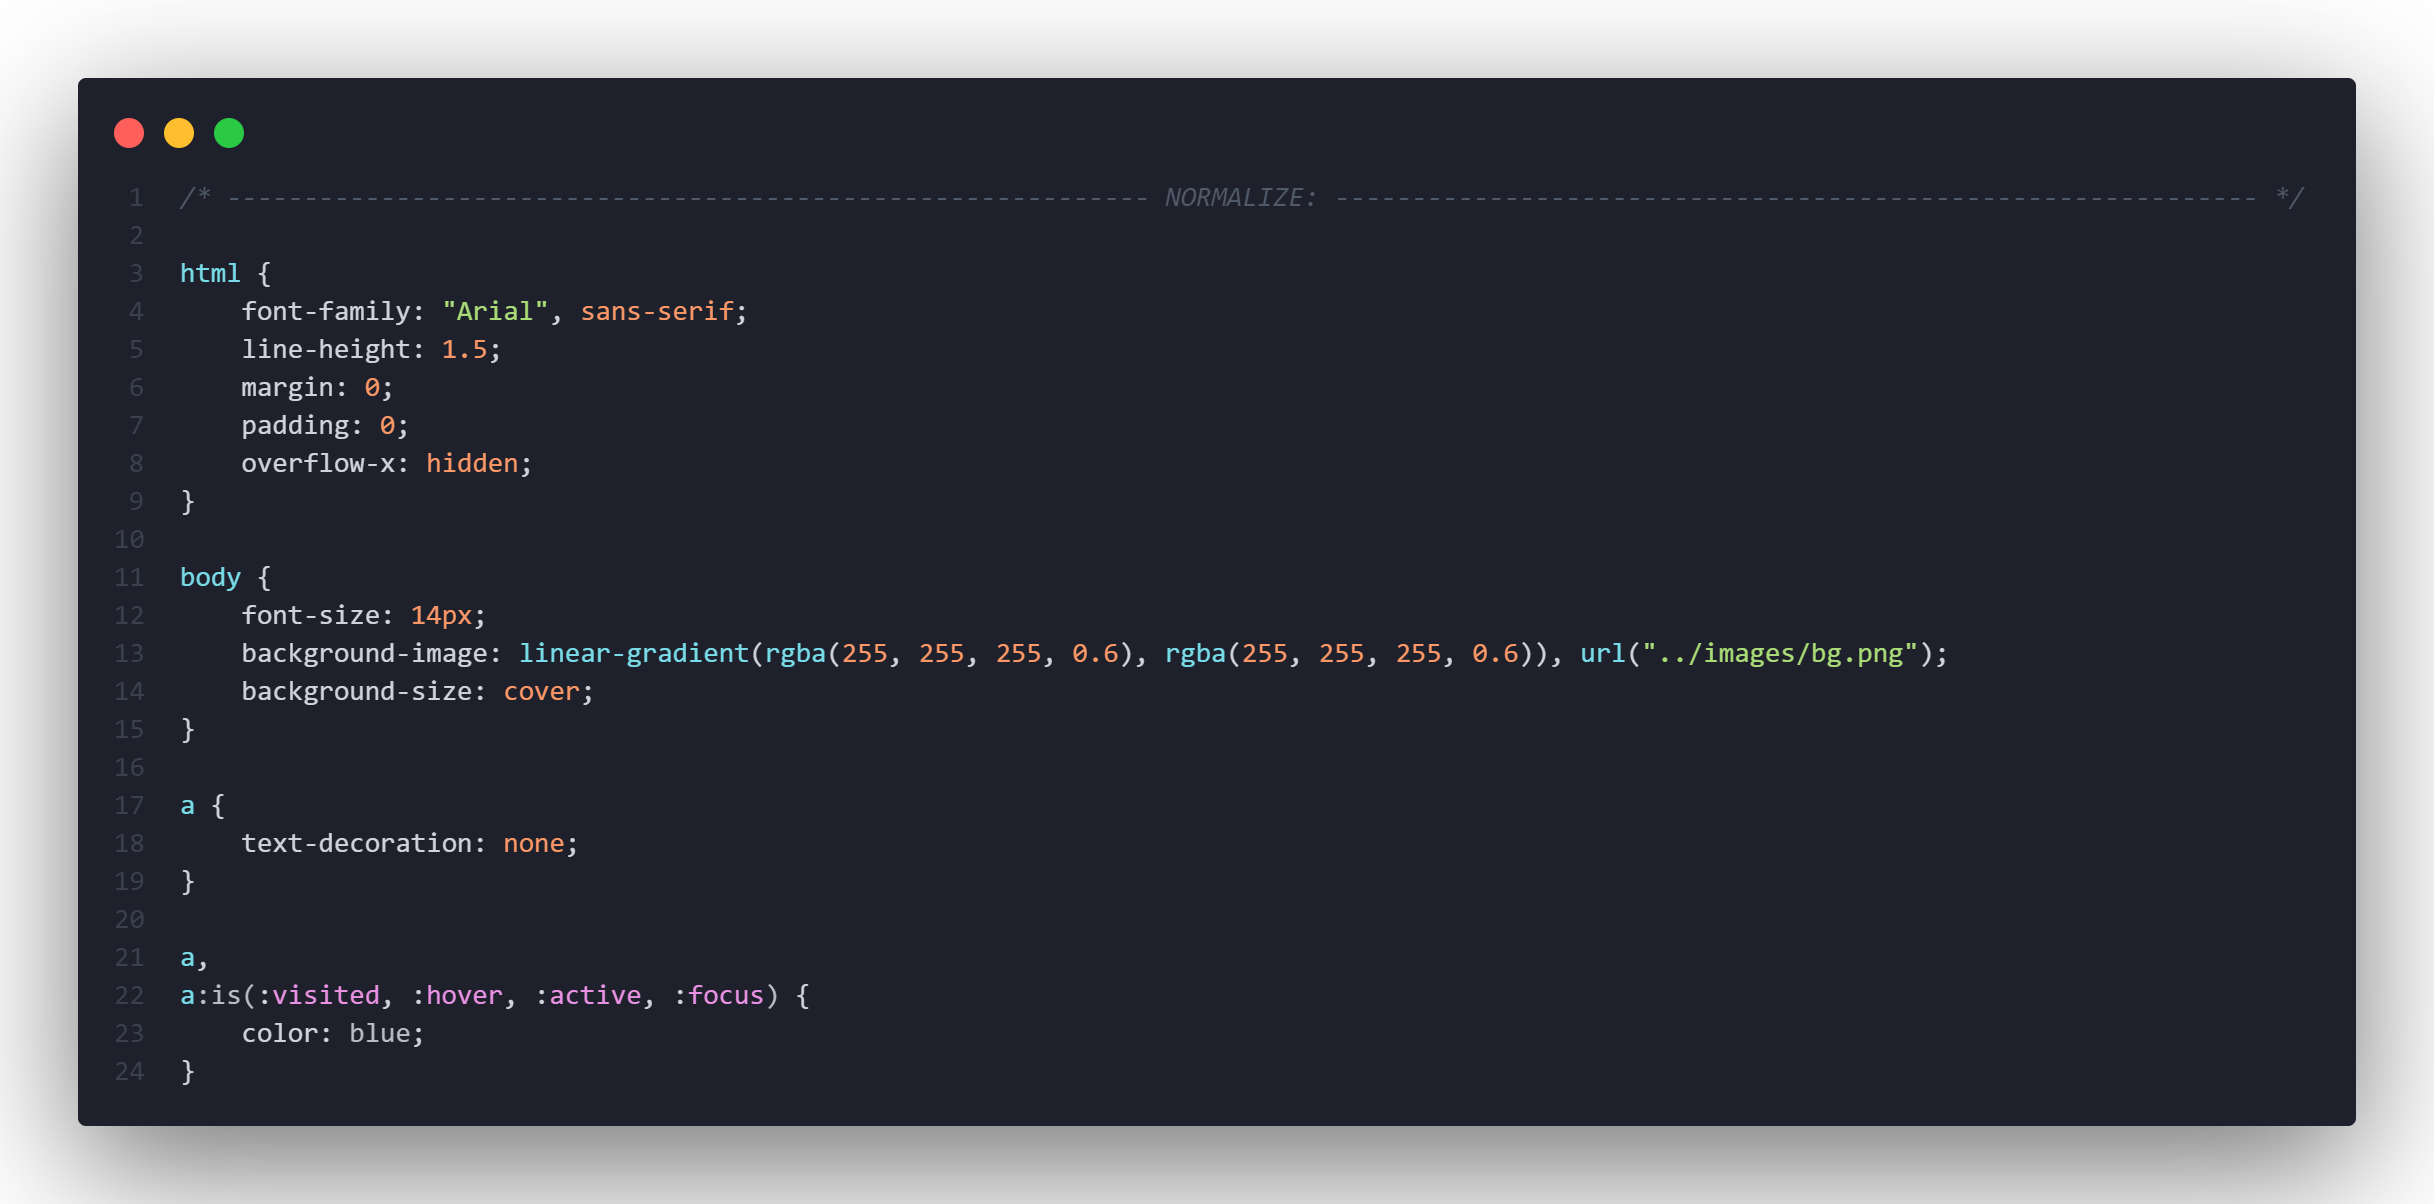
\includegraphics[width=10cm]{css.png}
    \centering
    \caption{Esempio di CSS utilizzato}
    \centering
\end{figure}

\subsubsection{JavaScript}

Per quanto riguarda JavaScript, ho implementato solo due funzioni di base per cambiare dinamicamente il contenuto di alcuni elementi quindi non ho avuto bisogno di nessuna libreria o framework.
\begin{figure}[h]
    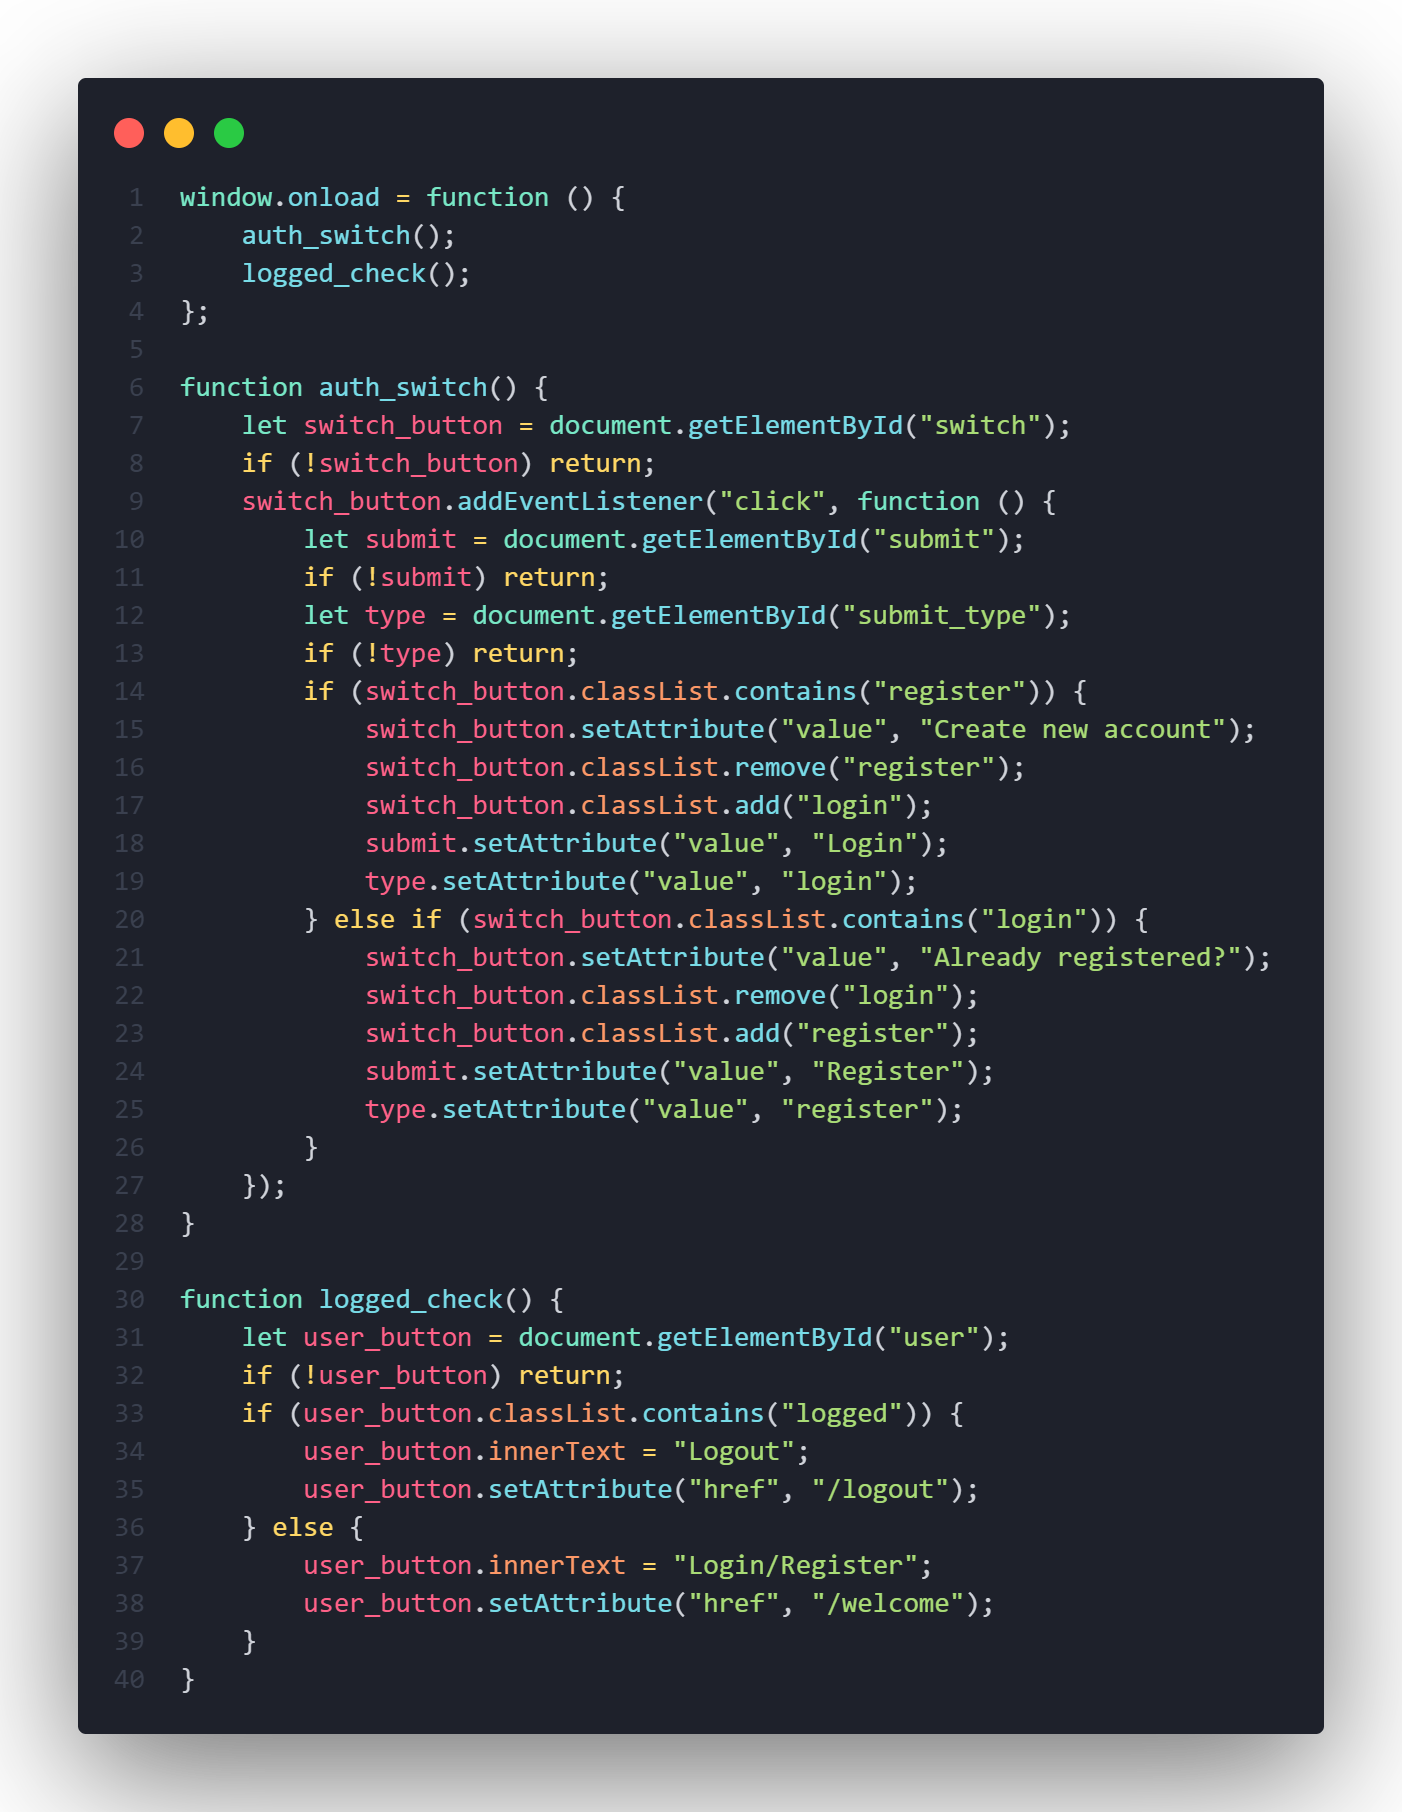
\includegraphics[width=10cm]{js.png}
    \centering
    \caption{Funzioni JavaScript utilizzate}
    \centering
\end{figure}

\newpage

% ------------------------------------------------------- Back-End -------------------------------------------------------

\subsection{Back-end}

\subsubsection{Funzionamento generale}

L'applicazione viene eseguita dal file \code{main.py} che richiama la funzione \code{create\_app()} del file \code{\_\_init\_\_.py} che crea l'applicazione Flask e la configura insieme al database, al login manager e ai blueprint. Dopodicché viene eseguita la funzione \code{run()} che avvia il server Flask. \\
All'interno del file \code{\_\_init\_\_.py} vengono inoltre registrati i blueprint che permettono di gestire le varie funzionalità dell'applicazione dai file \code{views.py} e \code{auth.py}.
\vskip 0.1cm
\begin{figure}[h]
    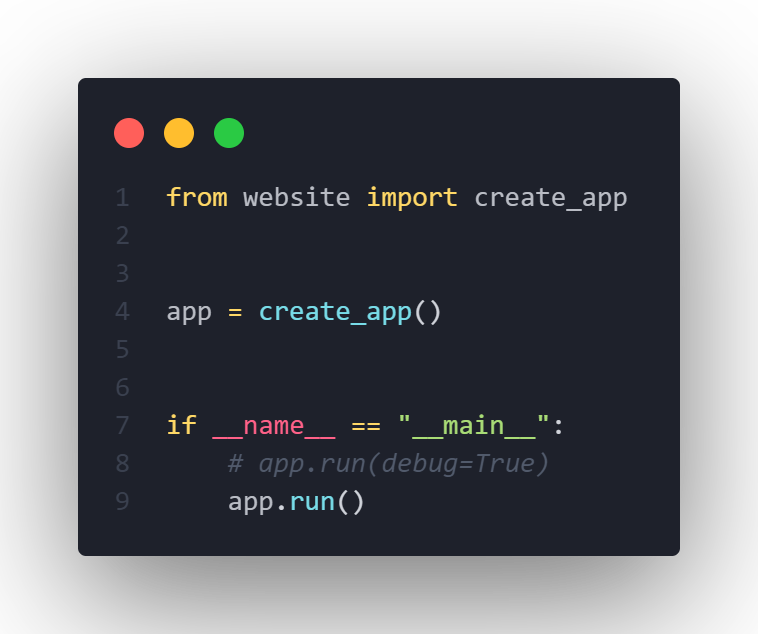
\includegraphics[width=6cm]{main.png}
    \centering
    \caption{\code{main.py}}
\end{figure}
\vskip 0.5cm
\noindent
Oltre a questi file, sono presenti anche i file \code{models.py}, che contiene la classe dell'oggetto che andrà inserito nel database, e \code{utils.py} che contiene alcune variabili a cui hanno accesso le view (sia generali sia quelle riguardanti l'autenticazione) che poi invieranno come parametri ai template HTML.
\vskip 0.1cm
\begin{figure}[h]
    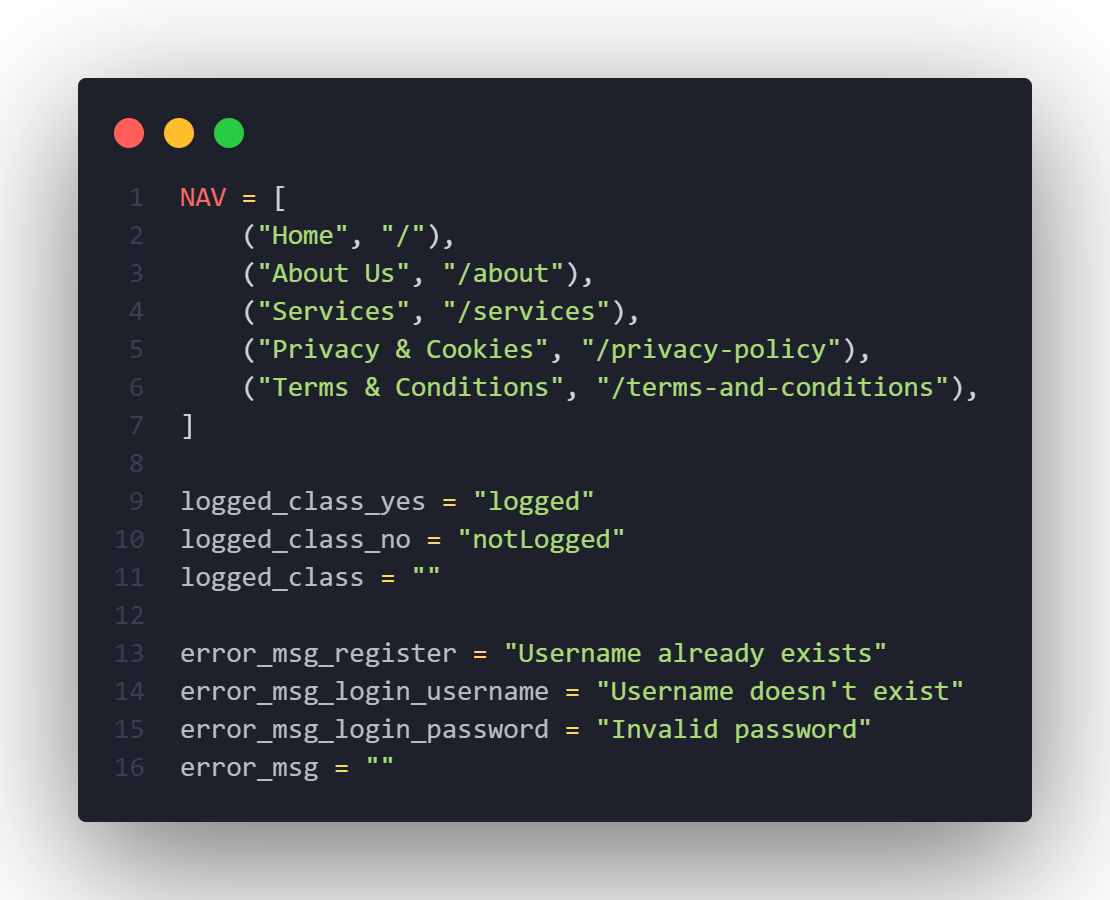
\includegraphics[width=7cm]{util.png}
    \centering
    \caption{\code{util.py}}
\end{figure}
\vskip 0.5cm
\noindent
Infine per quanto riguarda il download del PDF ho utilizzato la funzione \code{send\_file()} di Flask che permette di inviare un file al client.
\vskip 0.1cm
\begin{figure}[h]
    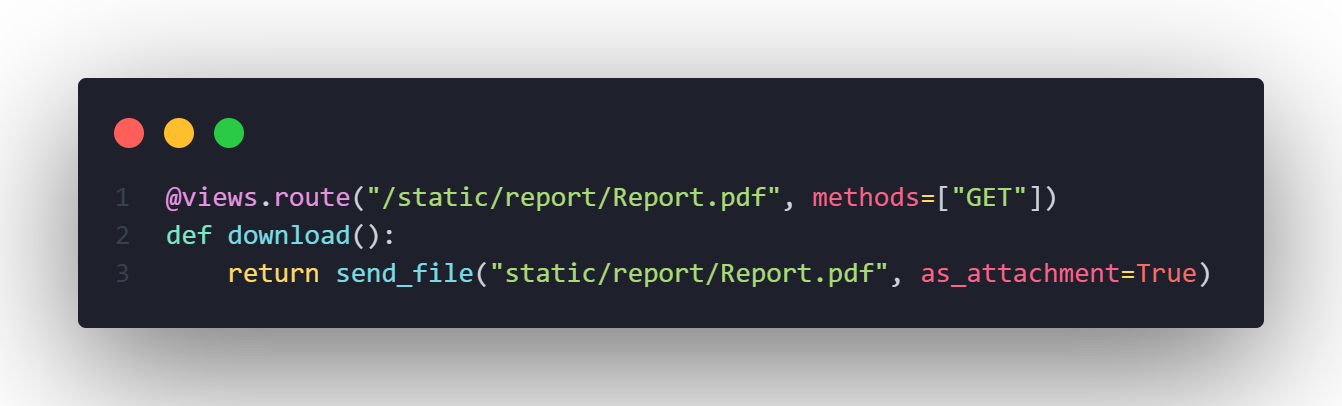
\includegraphics[width=10cm]{pdf.png}
    \centering
    \caption{Funzione per il download del PDF}
\end{figure}

\newpage

\subsubsection{Gestione view tramite Flask}

\begin{wrapfigure}[24]{r}{0.47\linewidth}
    \begin{minipage}{\linewidth}
        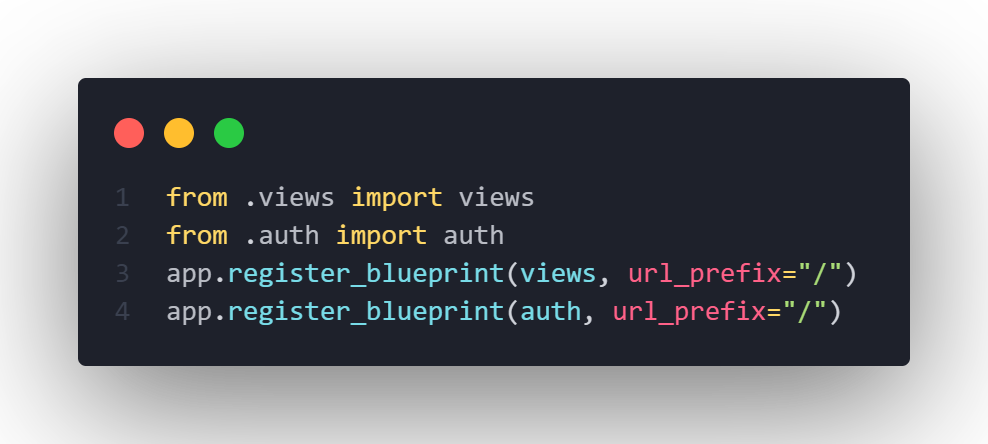
\includegraphics[width=8cm]{blueprints.png}
        \subcaption{Registrazione dei blueprint}
        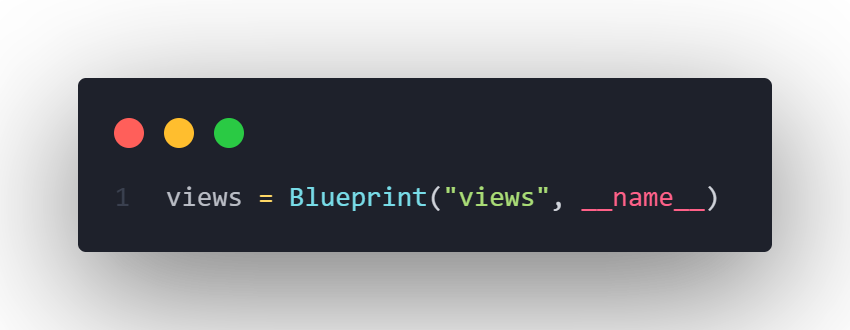
\includegraphics[width=8cm]{bp-views.png}
        \subcaption{Creazione del blueprint per le views}
        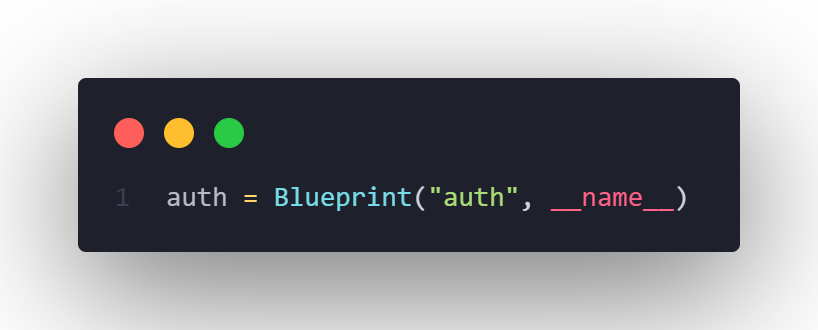
\includegraphics[width=8cm]{bp-auth.png}
        \subcaption{Creazione del blueprint per l'autenticazione}
    \end{minipage}
\end{wrapfigure}
\justifying
Come spiegato in precedenza, ho usato la libreria Flask, in particolare grazie hai suoi Blueprint (un meccanismo per separare diverse parti dell'applicazione in moduli riutilizzabili, serve a riorganizzare views e templates in modo da avere un codice più pulito e riutilizzabile, in questo modo è possibile organizzare l'app in diverse sezioni e utilizzare comunque la stessa struttura di routing). \\
I blueprint vengono creati tramite la funzione \code{Blueprint} che prende come parametri il nome del blueprint e il nome del package (nel mio caso \code{\_\_name\_\_}). Per poi registrare il blueprint all'interno dell'applicazione è necessario utilizzare la funzione \code{register\_blueprint} che prende come parametri il blueprint da registrare e il prefisso da utilizzare per le views del blueprint. \\
Per quanto riguarda poi l'effettiva creazione delle views e reindirizzamento del web server a tali view, ho utilizzato la funzione \code{route} propria delle view e dei blueprint di flask che prende come parametri il percorso della view e il metodo HTTP da utilizzare per accedere alla view e restituisce la funzione \code{render\_template} che prende come parametri il template da utilizzare e le variabili da passare al template. \\
\begin{figure}[h]
    \centering
    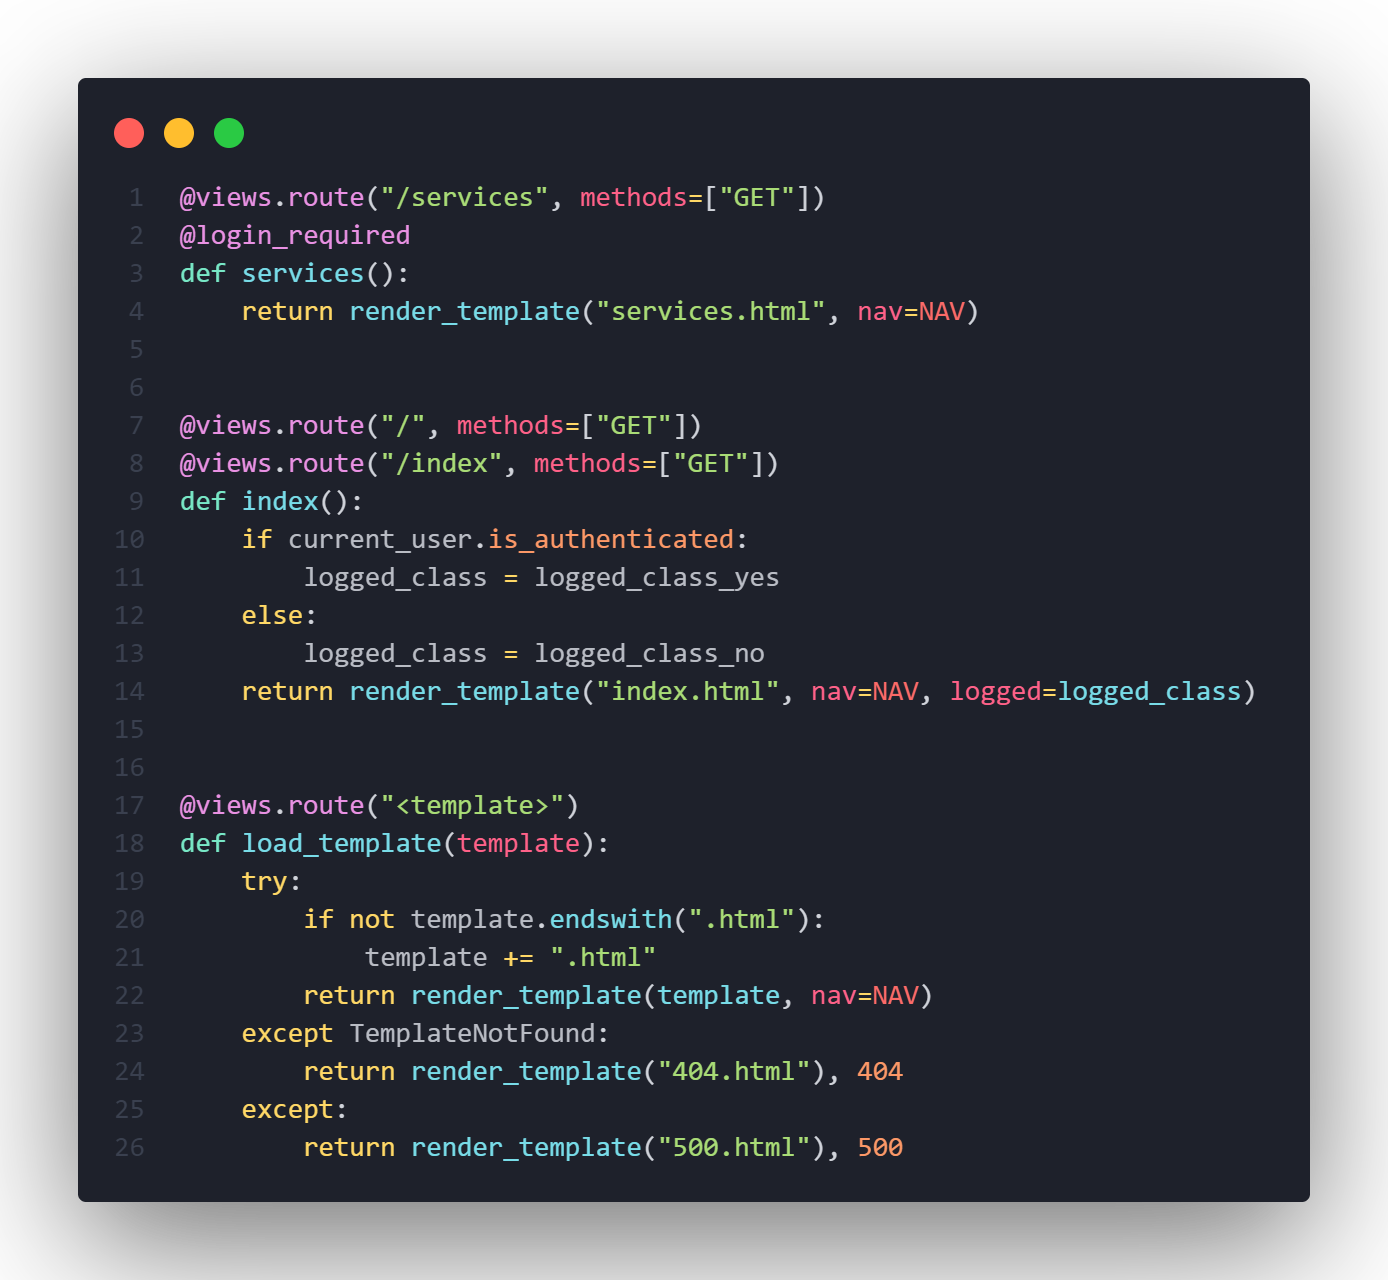
\includegraphics[width=12cm]{views.png}
    \caption{Esempio di implementazione delle view}
\end{figure}

\newpage

\subsubsection{Gestione database tramite flask\_sqlalchemy}

\begin{wrapfigure}[20]{r}{0.47\linewidth}
    \begin{minipage}{\linewidth}
        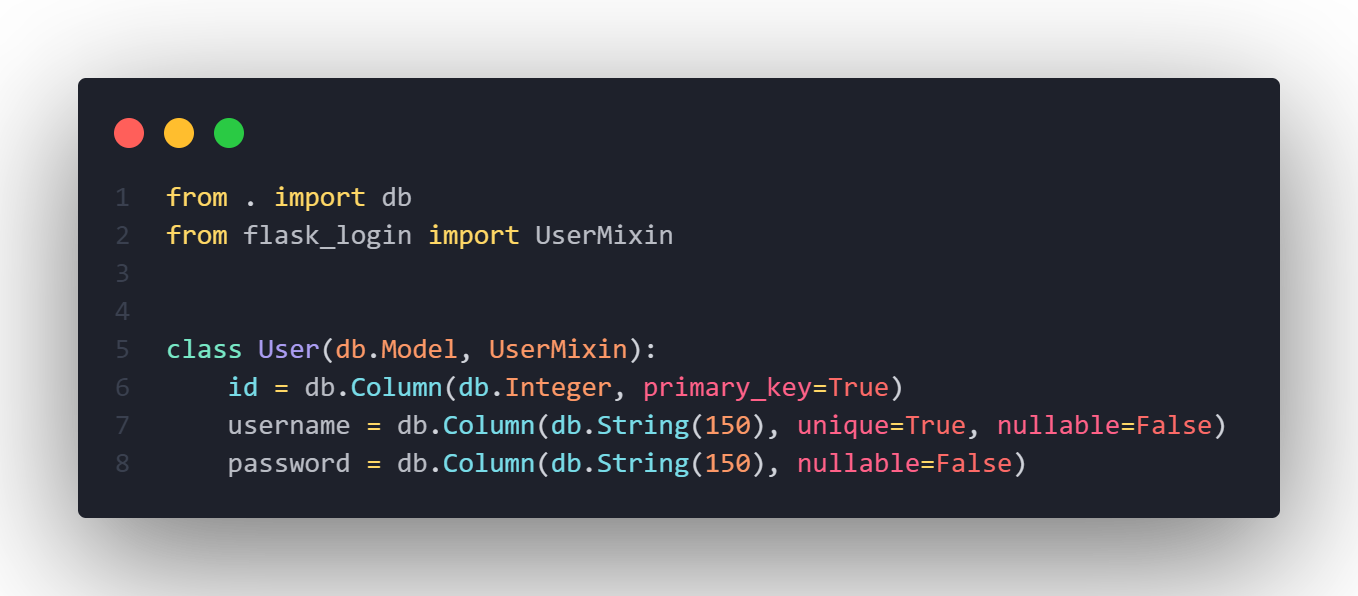
\includegraphics[width=8cm]{models.png}
        \subcaption{Modello del database}
        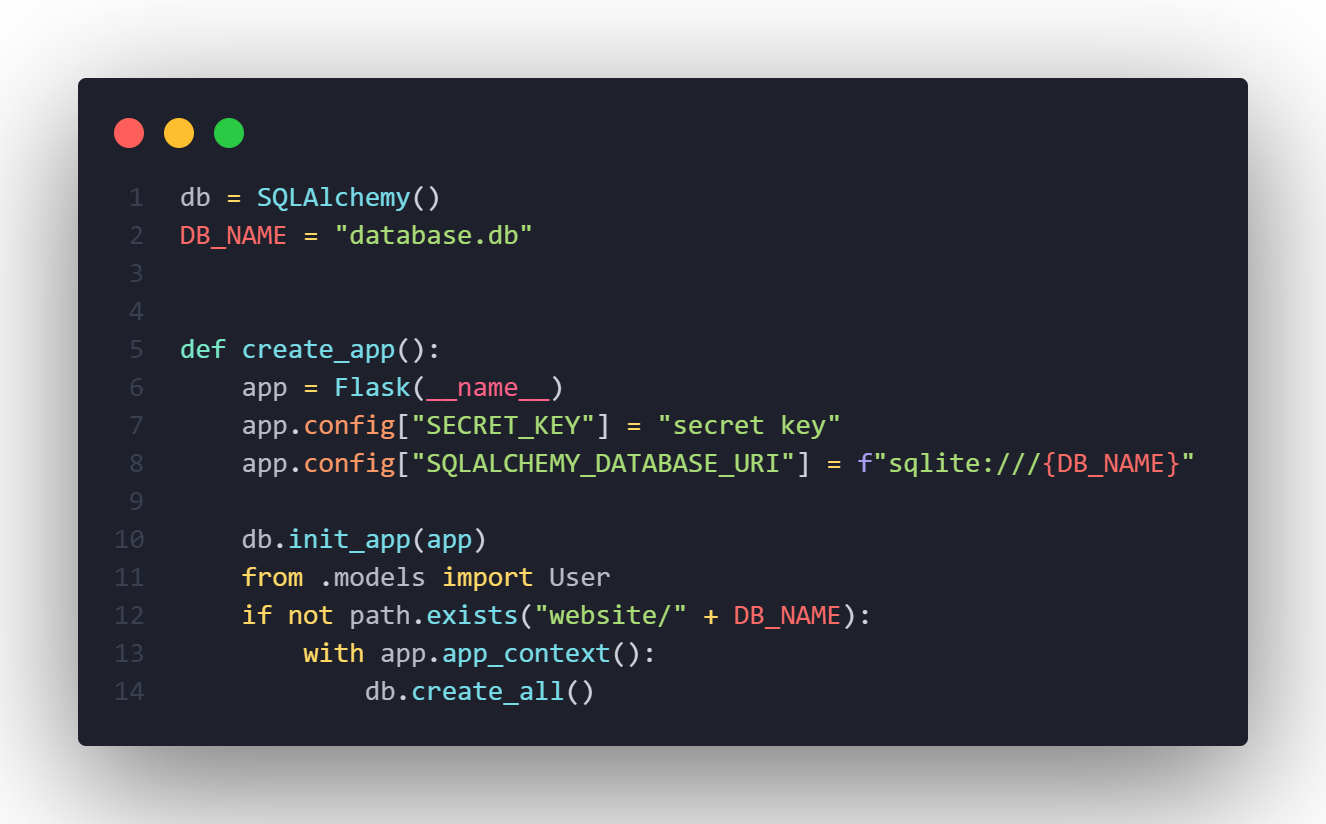
\includegraphics[width=8cm]{init-db.png}
        \subcaption{Inizializzazione del database}
    \end{minipage}
\end{wrapfigure}
\justifying
Per la gestione del database (che servirà poi per registrare i dati relativi all'autenticazione degli utenti) ho utilizzato la libreria flask\_sqlalchemy che permette di gestire il database tramite oggetti. L'immagine a destra mostra il file \code{models.py} che si occupa della creazione dell'oggetto User che andrà poi inserito all'interno del database. \\
Per quanto riguarda invece la sua inizializzazione, è gestita all'interno del file \code{\_\_init\_\_.py} che si occupa di creare il database (se non esiste già), di inizializzare la tabella \code{user} e di collegare il database all'app. \\
Sono riportati qui sotto alcuni esempi di utilizzo del database nell'applicazione: quali l'uso all'interno della funzione \code{load\_user} del \code{LoginManager} tramite una query che restituisce l'utente con l'id passato come parametro, l'uso di un'altra query sempre sulla tabella \code{User} per verificare se l'utente è già presente nel database, e infine l'effettiva creazione di un nuovo oggetto \code{User} e il suo inserimento nel database tramite la funzione \code{db.session.add} e \code{db.session.commit}.
\begin{figure}[h]
    \centering
    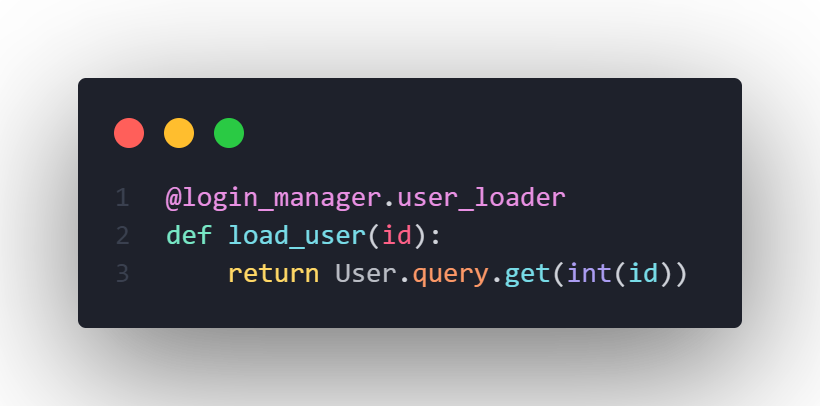
\includegraphics[width=8cm]{query-user.png}
    \caption{Query per ottenere l'utente con l'id passato come parametro}
\end{figure}
\vskip 0.3cm
\begin{figure}[h]
    \centering
    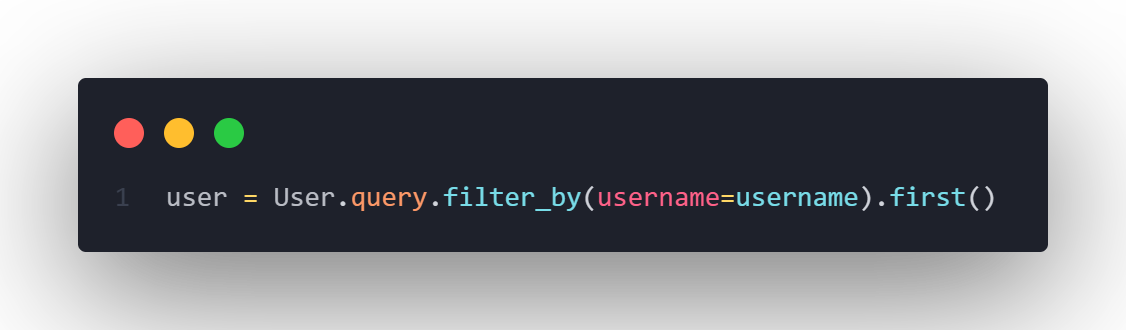
\includegraphics[width=10.5cm]{query.png}
    \caption{Query per verificare se l'utente è già presente nel database}
\end{figure}
\vskip 0.3cm
\begin{figure}[h]
    \centering
    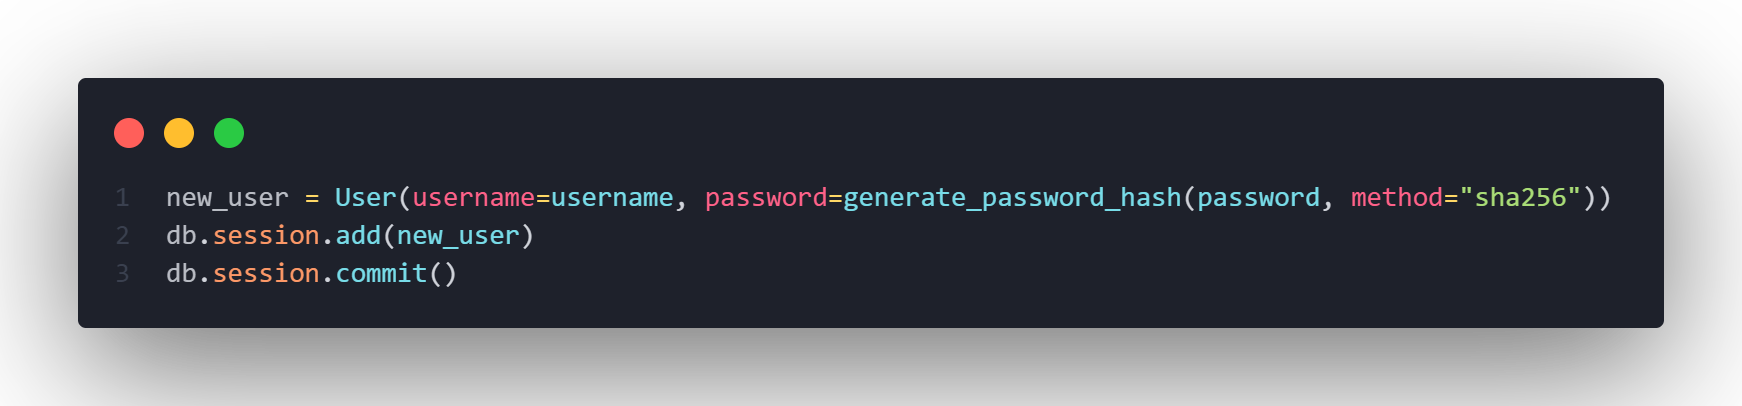
\includegraphics[width=16cm]{db-add.png}
    \caption{Creazione di un nuovo oggetto \code{User} e inserimento nel database}
\end{figure}

\subsubsection{Gestione autenticazione tramite flask\_login e werkzeug.security}

\begin{wrapfigure}[9]{r}{0.47\linewidth}
    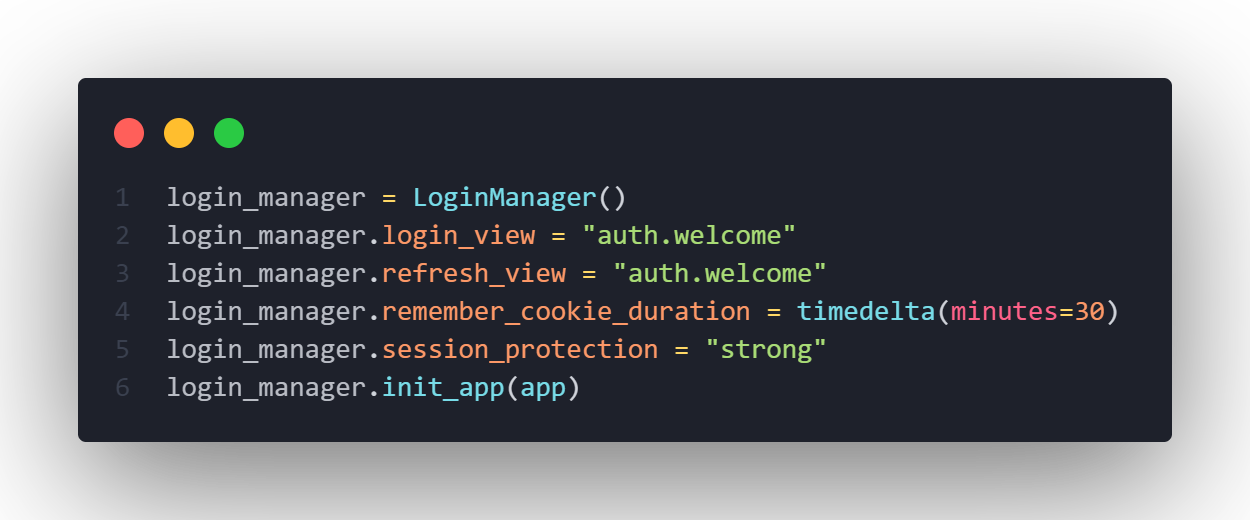
\includegraphics[width=8cm]{login-manager.png}
    \caption{Creazione del \code{LoginManager}}
\end{wrapfigure}
\justifying
Per quanto riguarda invece la gestione dell'autenticazione, ho utilizzato la libreria di flask \code{flask\_login} che permette di gestire l'autenticazione degli utenti. Per prima cosa è necessario creare un oggetto \code{LoginManager} (che io ho creato all'interno del file \code{\_\_init\_\_.py}) che si occupa di gestire l'autenticazione degli utenti. Dopo la sua creazione è possibile impostare alcune configurazioni: quali la \code{login\_view} che indica la view da reindirizzare in caso di utente non autenticato, la \code{refresh\_view} che indica la view da reindirizzare in caso di utente autenticato ma con sessione scaduta, \code{remember\_cookie\_duration} che indica la durata della sessione di un utente autenticato (e quindi la durata del cookie di autenticazione), \code{session\_protection} che indica il livello di protezione della sessione (in questo caso impostato a \code{strong} che indica che la sessione viene protetta da attacchi CSRF) e infine la funzione \code{load\_user} che ho spiegato in precedenza. \\
Inoltre è necessario fare in modo che l'oggetto \code{User} (che verrà poi utilizzato all'interno del database) estenda l'oggetto \code{UserMixin} (come si può vedere da un'immagine precedente), sempre facente parte della libreria \code{flask\_login}, che si occupa di gestire le informazioni dell'utente.
\justifying
\begin{figure}[h]
    \centering
    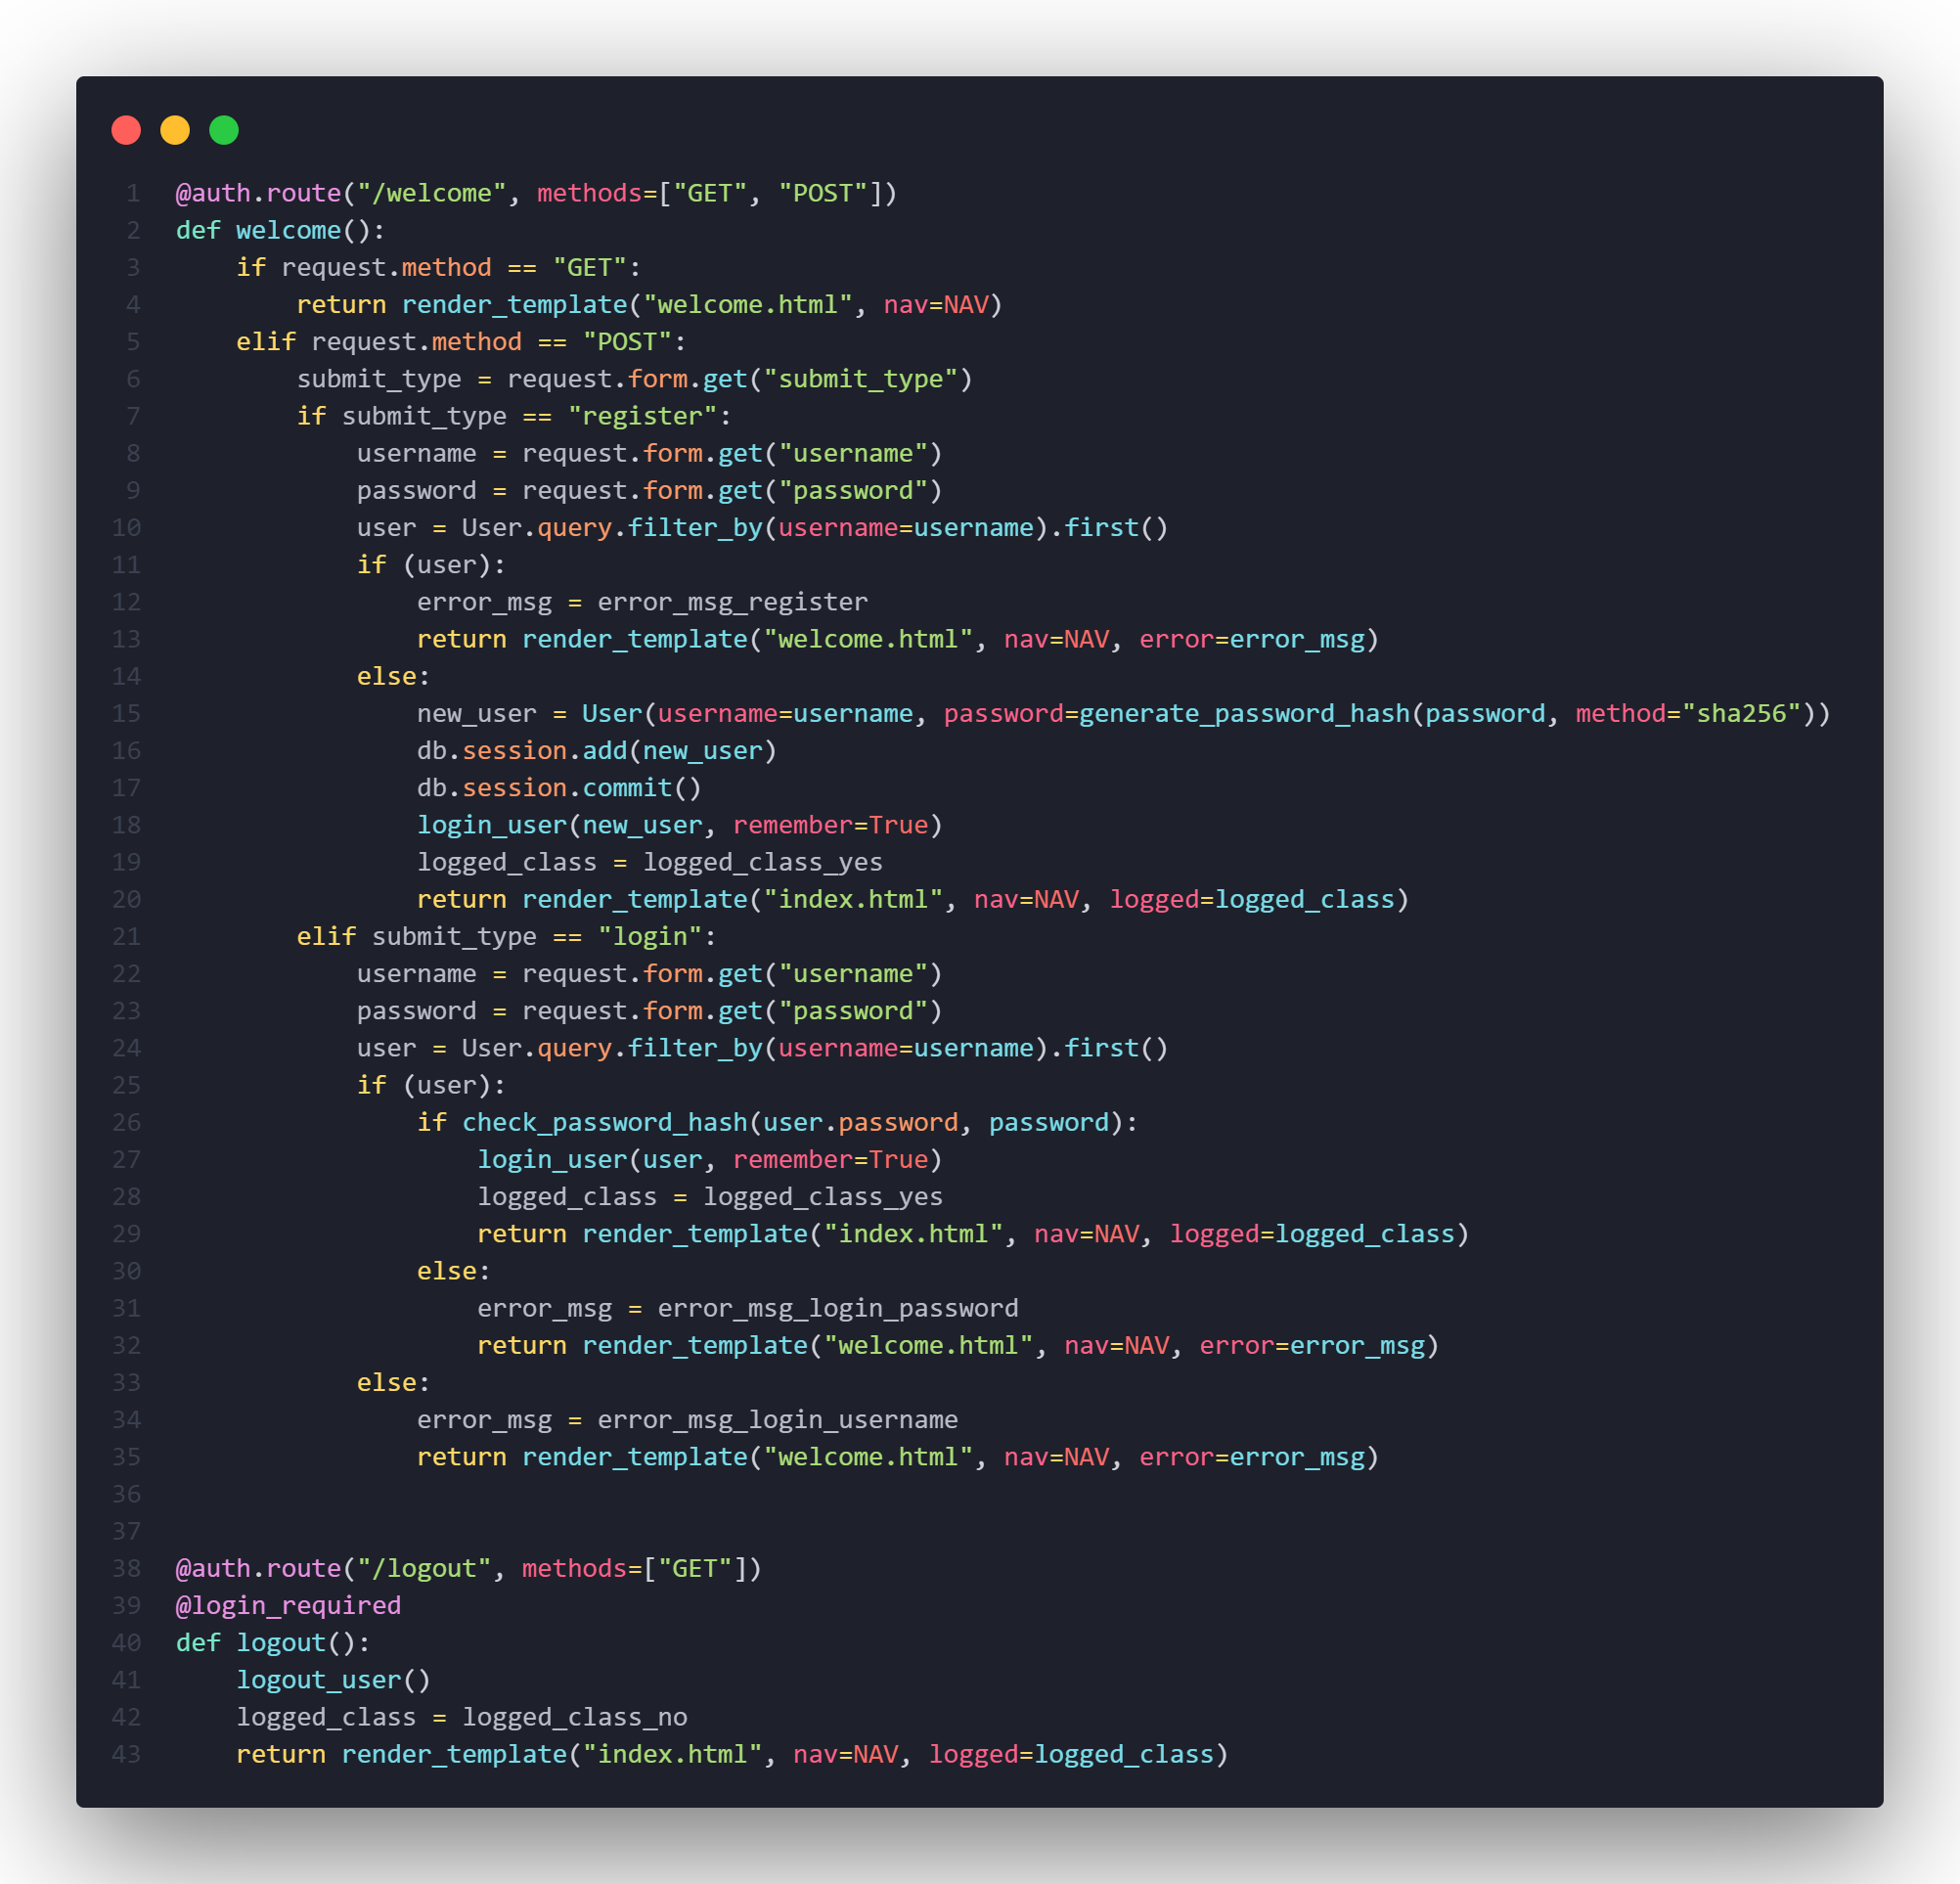
\includegraphics[width=12cm]{auth.png}
    \caption{Funzioni per l'autenticazione e il logout}
\end{figure}
\vskip 0.3cm
\noindent
Il modulo \code{flask\_login} permette di gestire l'autenticazione degli utenti tramite due funzioni: \code{login\_user} che permette di autenticare un utente e \code{logout\_user} che permette di invalidare la sessione di un utente. Inoltre permette anche di aggiungere un decorator \code{login\_required} che permette di reindirizzare l'utente alla \code{login\_view} impostata in precedenza in caso di utente non autenticato, e di accedere alle informazioni dell'utente tramite la variabile \code{current\_user} che contiene l'oggetto \code{User} dell'utente autenticato. \\
Infine per quanto riguarda la gestione della password, ho usato il modulo \code{werkzeug.security} che permette la gestione di hashing delle password. In particolare ho utilizzato la funzione \code{generate\_password\_hash} che permette di generare un hash della password passata come parametro (nello specifico si basa sull'algoritmo PBKDF2 e utilizza la funzione di hash SHA-256) e la funzione \code{check\_password\_hash} che permette di verificare se la password passata come parametro corrisponde al hash passato come secondo parametro. In questo modo è possibile salvare nel database l'hash della password invece che la password stessa, in modo da non doverla salvare in chiaro.
\vskip 1.5cm

\subsubsection{Gestione errori (status code)}

Durante l'esecuzione dell'applicazione sono tanti gli status code che possono venire restituiti dal server:
\begin{itemize}
    \item \code{200} \- OK: indica che la richiesta è stata elaborata con successo e che il server ha restituito una risposta corretta.
    \item \code{302} \- Found: indica che la risorsa richiesta è temporaneamente disponibile all'indirizzo specificato in un'intestazione di risposta "Location".
    \item \code{304} \- Not Modified: indica che la risorsa richiesta non è stata modificata dall'ultima volta che è stata richiesta e che il client può utilizzare la copia memorizzata nella cache.
    \item \code{404} \- Not Found: indica che la risorsa richiesta non è stata trovata sul server.
    \item \code{500} \- Internal Server Error: indica che si è verificato un errore interno sul server e che la richiesta non può essere elaborata.
\end{itemize}
Gli unici status code che dovrebbero essere restituiti dal server dovrebbero essere i primi tre, che indicano un esito positivo, tuttavia è possibile che durante l'esecuzione dell'applicazione si verifichino degli errori imprevisti come ad esempio un errore di tipo \code{404} se si cerca di accedere ad una pagina che non esiste o un errore di tipo \code{500} se si verifica un errore interno al server. \\
Per gestire questi errori è stato implementato un sistema di gestione degli errori che permette di ottenere una pagina di errore personalizzata in base al tipo di errore che si è verificato grazie all'uso del decoratore \code{errorhandler} dei blueprint di Flask (per quanto riguarda le view relative all'autenticazione) e grazie alla classe \code{TeplateNotFound} di Jinja2 (per quanto riguarda le view generali). \\
\begin{figure}[h]
    \centering
    \begin{subfigure}{.5\textwidth}
        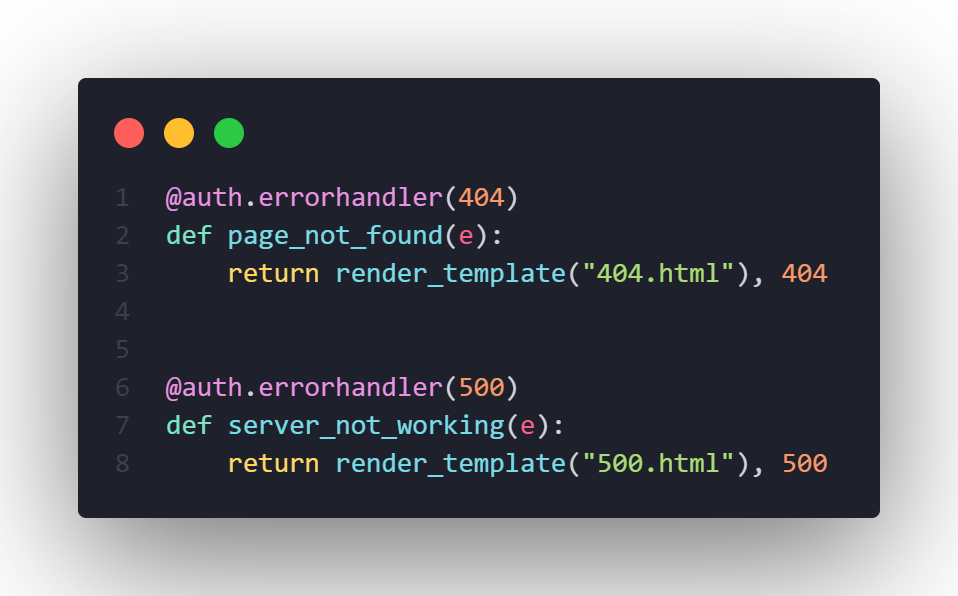
\includegraphics[width=8.5cm]{errorhandler.png}
        \caption{Gestione tramite \code{errorhandler}}
    \end{subfigure}%
    \begin{subfigure}{.5\textwidth}
        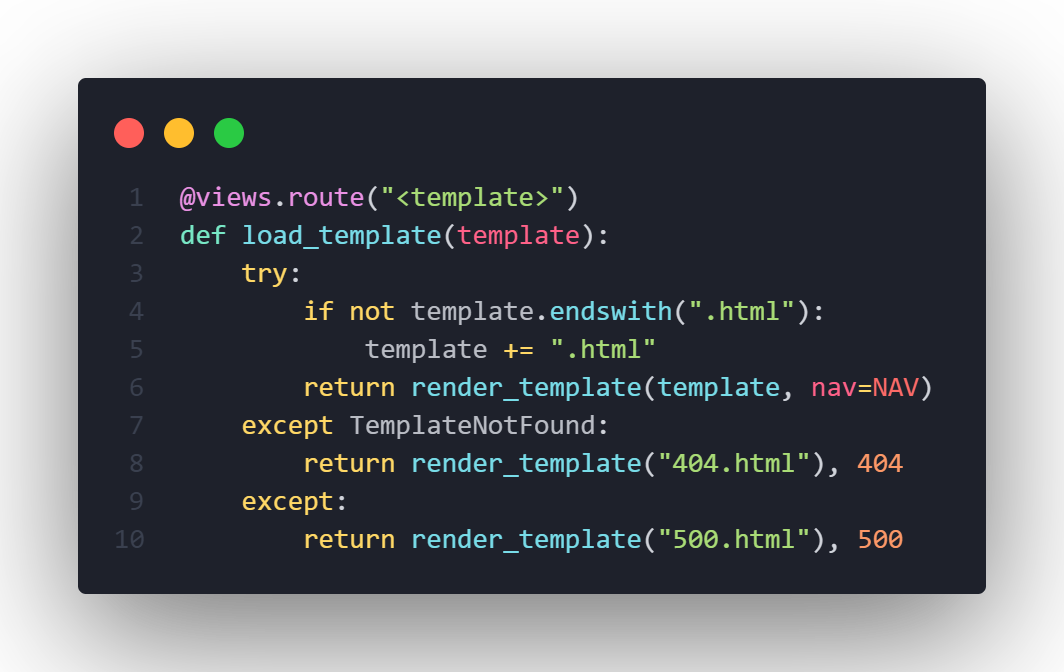
\includegraphics[width=8.5cm]{template-not-found.png}
        \caption{Gestione tramite \code{TemplateNotFound}}
    \end{subfigure}
\end{figure}

\newpage

% ------------------------------------------------------- ESECUZIONE -------------------------------------------------------

\section{Esecuzione}

Per eseguire il progetto è necessario seguire le istruzioni riportate nel file \code{README.md}:
\vskip 0.3cm
\begin{figure}[h]
    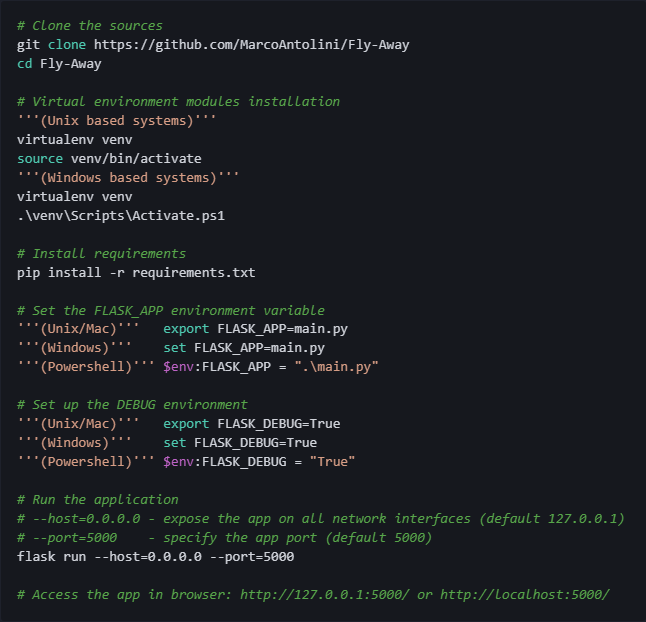
\includegraphics[width=13cm]{readme.png}
    \centering
\end{figure}
\vskip 0.5cm
\noindent
All'apertura del browser all'indirizzo \code{http://localhost:5000/} o \code{http://127.0.0.1:5000/} (o qualsiasi sia stato impostato) verrà visualizzata la pagina principale del web server:
\vskip 0.3cm
\begin{figure}[h]
    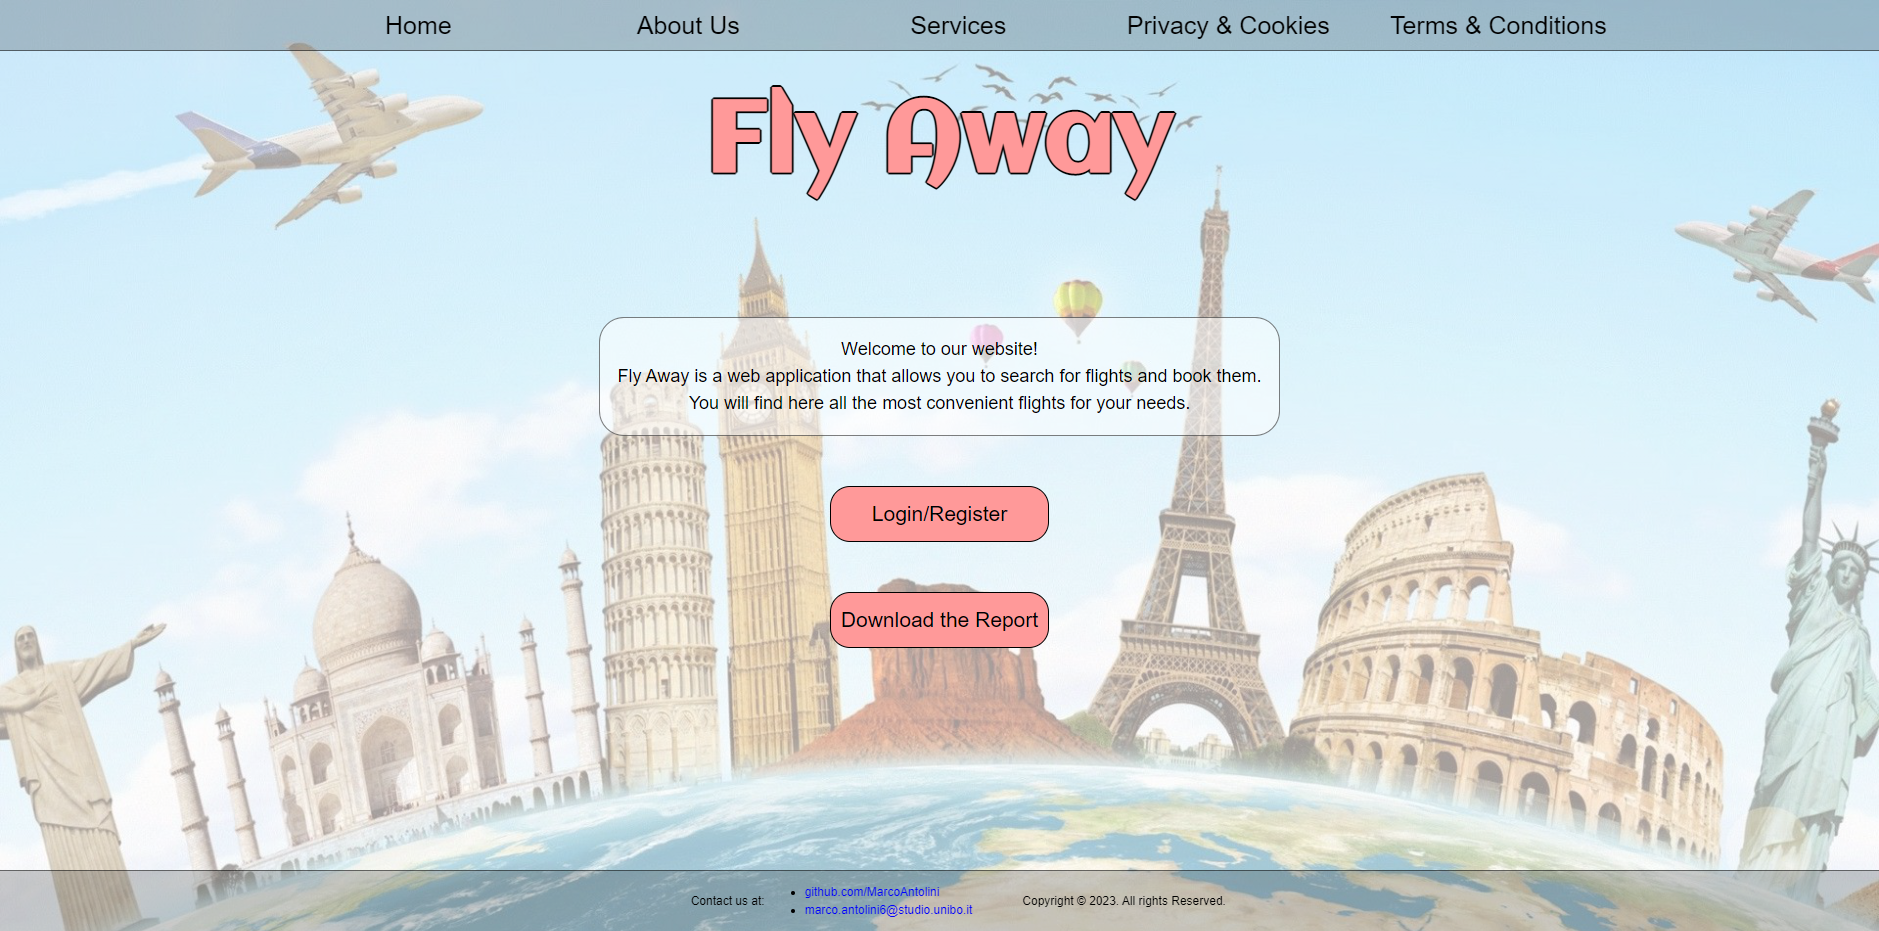
\includegraphics[width=17cm]{website.png}
    \centering
\end{figure}

\end{document}